In this assignment, you are to work with cyclic queues. A cyclic queue is a queue with fixed storage space allocated for it, such as an array of constant length, and two points pointing to the first and last element in the queue. As an example, consider a cyclic queue of length 8 as illustrated in \Cref{queueEmpty}.
\begin{figure}
  \subfigure[\label{queueEmpty}]{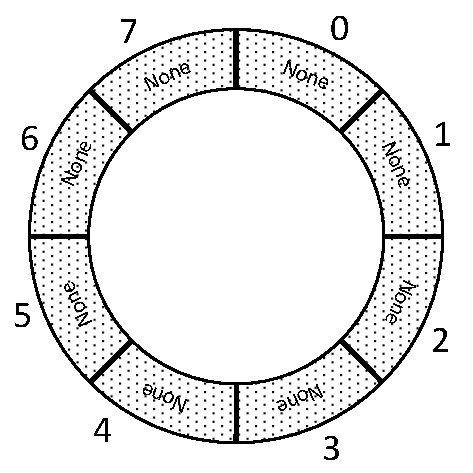
\includegraphics[]{queueEmpty}}
  \subfigure[\label{queue}]{
\includegraphics[]{queue}}
  \caption{A cyclic queue of length 8. Integers on the outside of the figure are position indices. (a) The initial state with no data and where the first and last are also set to \lstinline{None}. (b) A queue after enqueueing the sequence $7, 3, -1, 5$ and then dequeuing once such that the first element is 3 and the last is 5. The next element to be added will be in position 1.}
\end{figure}
When the queue maintains the variables \lstinline{first} and \lstinline{last}, where \lstinline{first} points to the position of the element in the front of the queue, and \lstinline{last} points to the position of the element in the back of the queue, which also is the last element added to the queue. Initially, point pointers are \lstinline{None}. If the queue is not full, then when enqueueing values to the queue, \lstinline{last} is cyclicly incremented by 1, and the value is stored in that position. If the queue is not empty, then dequeuing values from the queue, the value at position \lstinline{first} is returned and \lstinline{first} is cyclicly incremented by 1.

In this assignment, you are to make a module that implements the abstract datatype known as a \emph{cyclicQueue} for integers using imperative programming and which has the following interface \lstinline[language=console]{cyclicQueue.fsi}:
\begin{lstlisting}
module cyclicQueue

type Value = int

/// <summary>Create or clear the cyclic queue</summary>
/// <param name="n">The maximum number of elements</param>
val create: n: int -> unit

/// <summary>Add an element to the end of a queue</summary>
/// <param name="e">an element</param>
/// <returns>True if the queue had space for the element</returns>
val enqueue: e: Value -> bool

/// <summary>Remove the element in the front position of the queue</summary>
/// <returns>The first element in q or None if the queue is empty</returns>
val dequeue: unit -> Value option

/// <summary>Check if the queue is empty</summary>
/// <returns>True if the queue is empty</returns>
val isEmpty: unit -> bool

/// <summary>Get the length of the queue</summary>
/// <returns>The number of elements in the queue</returns>
val length: unit -> int

/// <summary>The queue on string form</summary>
/// <returns>A string representing the queue's elements</returns>
val toString: unit -> string
\end{lstlisting}
